\documentclass{standalone}
\usepackage{pgf,tikz}

\begin{document}

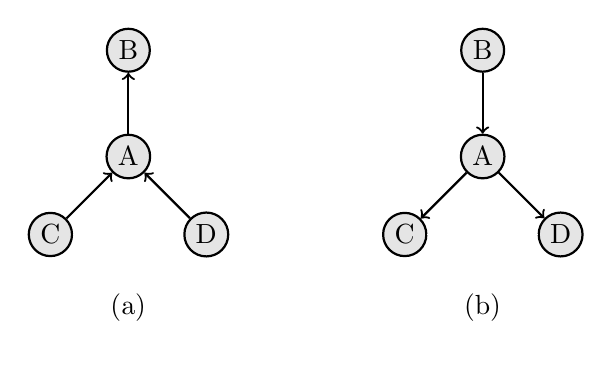
\begin{tikzpicture}
  [scale=0.45,every node/.style={circle,  thick, draw=black,fill=black!10,inner sep=2pt}]
  
  %%%%%%%%%%%%%%%%%%%%%% ROW 1 %%%%%%%%%%%%%%%%%%%%%% 
  

  
%   \node(cp1_1) at (0,0)  		{A};
%   \node(cp1_2) at (0,4)  		{B};
%   \node(cp1_3) at (-3,-3)      {C};
%   \node(cp1_4) at (3,-3)  		{D};
   
   \node(cp2_1) at (10,0)  		{A};
   \node(cp2_2) at (10,3)  		{B};
   \node(cp2_3) at (7.8,-2.2)       {C};
   \node(cp2_4) at (12.2,-2.2)  	{D};
   
   \node(cp3_1) at (20,0)  		{A};
   \node(cp3_2) at (20,3)  		{B};
   \node(cp3_3) at (17.8,-2.2)       {C};
   \node(cp3_4) at (22.2,-2.2)  	{D};
   
%  \foreach \fromcpA/\tocpA in {cp1_1/cp1_2,cp1_1/cp1_3,cp1_1/cp1_4}
%    \draw[<->, very thick] (\fromcpA) -- (\tocpA);
    
   \foreach \fromcpB/\tocpB in {cp2_1/cp2_2,cp2_3/cp2_1,cp2_4/cp2_1}
    \draw[->,  thick] (\fromcpB) -- (\tocpB);

	\foreach \fromcpC/\tocpC in {cp3_2/cp3_1,cp3_1/cp3_3,cp3_1/cp3_4}
    \draw[->,  thick] (\fromcpC) -- (\tocpC);
    
%       \draw[draw=white]  (cp1_3) -- (cp1_4) node [draw=none,fill=none,midway,below=15pt] {(a)};
	    \draw[draw=white]  (cp2_3) -- (cp2_4) node [draw=none,fill=none,midway,below=15pt] {(a)};
       	
       	 \draw[draw=white]  (cp3_3) -- (cp3_4) node [draw=none,fill=none,midway,below=15pt] {(b)};
       	
\end{tikzpicture}
\end{document}